\documentclass{article}
\usepackage[utf8]{inputenc}
\usepackage{amsmath, amssymb}
\usepackage{tcolorbox}
\usepackage{multicol}
\usepackage[a4paper, landscape, margin=1cm]{geometry}
\usepackage{tikz}

% Definir entorno para los cuadros con título negro
\newtcolorbox{teorema}[1]{
  colback=white,
  colframe=black,
  coltitle=white,
  colbacktitle=black,
  fonttitle=\bfseries,
  title={#1},
  boxrule=1pt,
  width=\linewidth,
  arc=2mm
}

\begin{document}

% ======================= PRIMERA PÁGINA ========================
\begin{center}
    \LARGE \textbf{Campo eléctrico y Corriente eléctrica}
\end{center}

\begin{multicols}{3}

% Primera columna
\begin{teorema}{Ley de Coulomb}
    $$\vec{F} = k\frac{|q_1q_2|}{r^2}[N] = k\frac{q_1q_2}{r^2}(\vec{r_1} - \vec{r_2}) [N]$$
    Variables y Unidades:
    \begin{itemize}
        \item $\vec{F}$: Fuerza eléctrica [$N$]
        \item $k$: Constante de Coulomb [$8,99 \times 10^9 \, N\cdot m^2/C^2$]
        \item $q_1$, $q_2$: Cargas eléctricas [$C$]
        \item $r$: Distancia entre cargas [$m$]
        \item $\vec{r_1}$, $\vec{r_2}$: Vectores posición [$m$]
    \end{itemize}
\end{teorema}

\begin{teorema}{Campo eléctrico}
    $$\vec{E} = k\frac{q_0}{r^2}\vec{r}\quad [\frac{N}{C}]$$
    Variables y Unidades:
    \begin{itemize}
        \item $\vec{E}$: Campo eléctrico [$N/C$]
        \item $k$: Constante de Coulomb [$N\cdot m^2/C^2$]
        \item $q_0$: Carga fuente [$C$]
        \item $r$: Distancia [$m$]
        \item $\vec{r}$: Vector dirección
    \end{itemize}
\end{teorema}

\begin{teorema}{Corriente en función de la densidad de carga}
    $$I = q \, n \, v_d \, S$$
    Variables y Unidades:
    \begin{itemize}
        \item $I$: Corriente [$A$]
        \item $q$: Carga de las partículas (densidad de partículas) [$C$]
        \item $n$: Densidad de partículas [$1/m^3$]
        \item $v_d$: Velocidad de deriva [$m/s$]
        \item $S$: Área de la sección transversal [$m^2$]
    \end{itemize}
\end{teorema}

\begin{teorema}{Potencial eléctrico}
    $$V = k\frac{q}{r} \quad [V]$$
    $$\vec{E} = -\nabla V$$
    Variables y Unidades:
    \begin{itemize}
        \item $V$: Potencial eléctrico [$V = J/C$]
        \item $q$: Carga fuente [$C$]
        \item $r$: Distancia [$m$]
        \item $\vec{E}$: Campo eléctrico [$N/C$]
    \end{itemize}
\end{teorema}

\begin{teorema}{Energía potencial eléctrica}
    $$U = k\frac{q_1 q_2}{r} \quad [J]$$
    Variables y Unidades:
    \begin{itemize}
        \item $U$: Energía potencial [$J$]
        \item $q_1$, $q_2$: Cargas [$C$]
        \item $r$: Distancia [$m$]
    \end{itemize}
\end{teorema}

% Segunda columna
\columnbreak

\begin{teorema}{Ley de Gauss (eléctrico)}
    $$\oint \vec{E} \cdot d\vec{S} = \frac{Q_{\text{int}}}{\epsilon_0}$$
    Variables y Unidades:
    \begin{itemize}
        \item $\vec{E}$: Campo eléctrico [$N/C$]
        \item $d\vec{S}$: Elemento de superficie [$m^2$]
        \item $Q_{\text{int}}$: Carga interna [$C$]
        \item $\epsilon_0$: Permitividad del vacío [$F/m$]
    \end{itemize}
\end{teorema}

\begin{teorema}{Capacidad de un condensador plano}
    $$C = \frac{\epsilon_0 S}{d} \quad [F]$$
    Variables y Unidades:
    \begin{itemize}
        \item $C$: Capacidad [$F$]
        \item $\epsilon_0$: Permitividad del vacío [$F/m$]
        \item $S$: Superficie de las placas [$m^2$]
        \item $d$: Distancia entre placas [$m$]
    \end{itemize}
\end{teorema}

\begin{teorema}{Capacidad (general)}
    $$C = \frac{Q}{V} \quad [F]$$
    Variables y Unidades:
    \begin{itemize}
        \item $C$: Capacidad [$F$]
        \item $Q$: Carga almacenada [$C$]
        \item $V$: Voltaje [$V$]
    \end{itemize}
\end{teorema}

\begin{teorema}{Energía almacenada en un condensador}
    $$U = \frac{1}{2} C V^2$$
    Variables y Unidades:
    \begin{itemize}
        \item $U$: Energía [$J$]
        \item $C$: Capacidad [$F$]
        \item $V$: Voltaje [$V$]
    \end{itemize}
\end{teorema}

\begin{teorema}{Asociación de capacitores}
    Serie: $$\frac{1}{C_{\text{eq}}} = \sum_i \frac{1}{C_i}$$
    Paralelo: $$C_{\text{eq}} = \sum_i C_i$$
    Variables y Unidades:
    \begin{itemize}
        \item $C_{\text{eq}}$: Capacidad equivalente [$F$]
        \item $C_i$: Capacidades individuales [$F$]
    \end{itemize}
\end{teorema}

% Tercera columna
\columnbreak

\begin{teorema}{Corriente eléctrica}
    $$ I = \frac{Q}{t} \quad [A]$$
    Variables y Unidades:
    \begin{itemize}
        \item $I$: Corriente [$A$]
        \item $Q$: Carga [$C$]
        \item $t$: Tiempo [$s$]
    \end{itemize}
\end{teorema}

\begin{teorema}{Densidad de corriente}
    $$\vec{J} = \sigma \vec{E}$$
    Variables y Unidades:
    \begin{itemize}
        \item $\vec{J}$: Densidad de corriente [$A/m^2$]
        \item $\sigma$: Conductividad [$S/m$]
        \item $\vec{E}$: Campo eléctrico [$N/C$]
    \end{itemize}
\end{teorema}

\begin{teorema}{Ley de Ohm (microscópica)}
    $$\vec{E} = \rho \vec{J}$$
    $$V = IR$$
    Variables y Unidades:
    \begin{itemize}
        \item $\vec{E}$: Campo eléctrico [$N/C$]
        \item $\rho$: Resistividad [$\Omega \cdot m$]
        \item $\vec{J}$: Densidad de corriente [$A/m^2$]
        \item $V$: Voltaje [$V$]
        \item $I$: Corriente [$A$]
        \item $R$: Resistencia [$\Omega$]
    \end{itemize}
\end{teorema}

\begin{teorema}{Resistencia}
    $$R = \rho \frac{L}{S}$$
    Variables y Unidades:
    \begin{itemize}
        \item $R$: Resistencia [$\Omega$]
        \item $\rho$: Resistividad [$\Omega \cdot m$]
        \item $L$: Longitud [$m$]
        \item $S$: Superficie [$m^2$]
    \end{itemize}
\end{teorema}

\begin{teorema}{Relación entre resistividad y conductividad}
    $$\rho = \frac{1}{\sigma} \quad \text{y} \quad \sigma = n \, q \, \mu$$
    Variables y Unidades:
    \begin{itemize}
        \item $\rho$: Resistividad [$\Omega \cdot m$]
        \item $\sigma$: Conductividad [$S/m$]
        \item $n$: Densidad de partículas cargadas [$1/m^3$]
        \item $q$: Carga de las partículas [$C$]
        \item $\mu$: Movilidad de las partículas cargadas [$m^2/V \cdot s$]
    \end{itemize}
\end{teorema}

\begin{teorema}{Potencia eléctrica}
    $$P = I V = I^2 R = \frac{V^2}{R}$$
    Variables y Unidades:
    \begin{itemize}
        \item $P$: Potencia [$W$]
        \item $V$: Voltaje [$V$]
        \item $I$: Corriente [$A$]
        \item $R$: Resistencia [$\Omega$]
    \end{itemize}
\end{teorema}

\end{multicols}

% ======================= SEGUNDA PÁGINA ========================
\newpage

\begin{center}
    \LARGE \textbf{Campo magnético}
\end{center}

\begin{multicols}{3}

% Primera columna
\begin{teorema}{Campo magnético de un hilo recto}
    $$B = \frac{\mu_0 I}{2\pi r}$$
    Variables y Unidades:
    \begin{itemize}
        \item $B$: Campo magnético [$T$]
        \item $\mu_0$: Permeabilidad [$4\pi \times 10^{-7} \, T\cdot m/A$]
        \item $I$: Corriente [$A$]
        \item $r$: Distancia [$m$]
    \end{itemize}
\end{teorema}

\begin{teorema}{Campo magnético de un solenoide}
    $$B = \mu_0 n I$$
    Variables y Unidades:
    \begin{itemize}
        \item $B$: Campo magnético [$T$]
        \item $\mu_0$: Permeabilidad [$T\cdot m/A$]
        \item $n$: Vueltas por unidad de longitud [$1/m$]
        \item $I$: Corriente [$A$]
    \end{itemize}
\end{teorema}

\begin{teorema}{Ley de Gauss para el magnetismo}
    $$\oint \vec{B} \cdot d\vec{S} = 0$$
    Variables y Unidades:
    \begin{itemize}
        \item $\vec{B}$: Campo magnético [$T$]
        \item $d\vec{S}$: Superficie [$m^2$]
    \end{itemize}
\end{teorema}

% Segunda columna
\columnbreak

\begin{teorema}{Ley de Ampère}
    $$\oint \vec{B} \cdot d\vec{l} = \mu_0 I_{\text{int}}$$
    Variables y Unidades:
    \begin{itemize}
        \item $\vec{B}$: Campo magnético [$T$]
        \item $d\vec{l}$: Elemento de longitud [$m$]
        \item $\mu_0$: Permeabilidad [$T\cdot m/A$]
        \item $I_{\text{int}}$: Corriente interna [$A$]
    \end{itemize}
\end{teorema}

\begin{teorema}{Fuerza de Lorentz}
    $$\vec{F} = q(\vec{E} + \vec{v} \times \vec{B})$$
    Variables y Unidades:
    \begin{itemize}
        \item $\vec{F}$: Fuerza [$N$]
        \item $q$: Carga [$C$]
        \item $\vec{E}$: Campo eléctrico [$N/C$]
        \item $\vec{v}$: Velocidad [$m/s$]
        \item $\vec{B}$: Campo magnético [$T$]
    \end{itemize}

    \begin{center}
        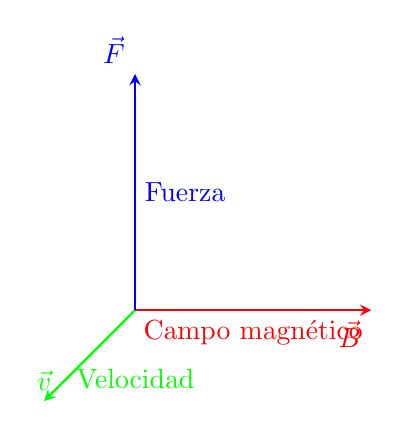
\begin{tikzpicture}[scale=1.5, >=stealth]
            % Ejes coordenados
            \draw[->, thick, green] (0,0,0) -- (0,0,2) node[anchor=south] {\textcolor{green}{$\vec{v}$}};
            \draw[->, thick, red] (0,0,0) -- (2,0,0) node[anchor=north east] {\textcolor{red}{$\vec{B}$}};
            \draw[->, thick, blue] (0,0,0) -- (0,2,0) node[anchor=south east] {\textcolor{blue}{$\vec{F}$}};

            % Etiquetas
            \node[anchor=north] at (1,0,0) {\textcolor{red}{Campo magnético}};
            \node[anchor=west] at (0,1,0) {\textcolor{blue}{Fuerza}};
            \node[anchor=west] at (0,0,1.5) {\textcolor{green}{Velocidad}};
        \end{tikzpicture}
    \end{center}
\end{teorema}

\begin{teorema}{Fuerza sobre un conductor}
    $$\vec{F} = I \vec{L} \times \vec{B}$$
    Variables y Unidades:
    \begin{itemize}
        \item $\vec{F}$: Fuerza [$N$]
        \item $I$: Corriente [$A$]
        \item $\vec{L}$: Vector longitud [$m$]
        \item $\vec{B}$: Campo magnético [$T$]
    \end{itemize}
\end{teorema}

% Tercera columna
\columnbreak

\begin{teorema}{Ley de Faraday}
    $$\mathcal{E} = -\frac{d\Phi_B}{dt}$$
    $$\Phi_B = \int \vec{B} \cdot d\vec{S}$$
    Variables y Unidades:
    \begin{itemize}
        \item $\mathcal{E}$: Fem inducida [$V$]
        \item $\Phi_B$: Flujo magnético [$Wb$]
        \item $\vec{B}$: Campo magnético [$T$]
        \item $d\vec{S}$: Superficie [$m^2$]
    \end{itemize}
\end{teorema}

\begin{teorema}{Inductancia}
    $$\mathcal{E} = -L \frac{dI}{dt}$$
    Variables y Unidades:
    \begin{itemize}
        \item $\mathcal{E}$: Fem inducida [$V$]
        \item $L$: Inductancia [$H$]
        \item $I$: Corriente [$A$]
    \end{itemize}
\end{teorema}

\begin{teorema}{Energía en campo magnético}
    $$U = \frac{1}{2} L I^2$$
    Variables y Unidades:
    \begin{itemize}
        \item $U$: Energía [$J$]
        \item $L$: Inductancia [$H$]
        \item $I$: Corriente [$A$]
    \end{itemize}
\end{teorema}

\end{multicols}

% ======================= TERCERA PÁGINA ========================
\newpage

\begin{center}
    \LARGE \textbf{Ondas}
\end{center}

\begin{multicols}{3}

% Primera columna
\begin{teorema}{Relación energía y frecuencia}
    $$E = h \nu$$
    Variables y Unidades:
    \begin{itemize}
        \item $E$: Energía [$J$]
        \item $h$: Constante de Planck [$6.626 \times 10^{-34} \, J \cdot s$]
        \item $\nu$: Frecuencia [$Hz$]
    \end{itemize}
\end{teorema}

\begin{teorema}{Relación velocidad, frecuencia y longitud de onda}
    $$c = f \lambda$$
    Variables y Unidades:
    \begin{itemize}
        \item $c$: Velocidad de la onda [$m/s$]
        \item $f$: Frecuencia [$Hz$]
        \item $\lambda$: Longitud de onda [$m$]
    \end{itemize}
\end{teorema}

\begin{teorema}{Función de onda}
    $$y(x,t) = A \sin(kx - \omega t + \phi)$$
    Variables y Unidades:
    \begin{itemize}
        \item $y(x,t)$: Desplazamiento [$m$]
        \item $A$: Amplitud [$m$]
        \item $k$: Número de onda [$rad/m$]
        \item $\omega$: Frecuencia angular [$rad/s$]
        \item $\phi$: Fase inicial [$rad$]
    \end{itemize}
\end{teorema}

\end{multicols}

% ======================= NUEVO APARTADO: CIRCUITOS ========================
\newpage

\begin{center}
    \LARGE \textbf{Circuitos Eléctricos}
\end{center}

\begin{multicols}{3}

% Primera columna
\begin{teorema}{Ley de Ohm}
    $$V = I R$$
    Variables y Unidades:
    \begin{itemize}
        \item $V$: Voltaje [$V$]
        \item $I$: Corriente [$A$]
        \item $R$: Resistencia [$\Omega$]
    \end{itemize}
\end{teorema}

\begin{teorema}{Potencia eléctrica}
    $$P = I V = I^2 R = \frac{V^2}{R}$$
    Variables y Unidades:
    \begin{itemize}
        \item $P$: Potencia [$W$]
        \item $V$: Voltaje [$V$]
        \item $I$: Corriente [$A$]
        \item $R$: Resistencia [$\Omega$]
    \end{itemize}
\end{teorema}

% Segunda columna
\columnbreak

\begin{teorema}{Ley de Kirchhoff de Corrientes (LKC)}
    $$\sum I_{\text{entrante}} = \sum I_{\text{saliente}}$$
    Variables y Unidades:
    \begin{itemize}
        \item $I$: Corriente [$A$]
    \end{itemize}
\end{teorema}

\begin{teorema}{Ley de Kirchhoff de Tensiones (LKT)}
    $$\sum V = 0$$
    Variables y Unidades:
    \begin{itemize}
        \item $V$: Voltaje [$V$]
    \end{itemize}
\end{teorema}

% Tercera columna
\columnbreak

\begin{teorema}{Asociación de resistencias}
    Serie: $$R_{\text{eq}} = \sum_i R_i$$
    Paralelo: $$\frac{1}{R_{\text{eq}}} = \sum_i \frac{1}{R_i}$$
    Variables y Unidades:
    \begin{itemize}
        \item $R_{\text{eq}}$: Resistencia equivalente [$\Omega$]
        \item $R_i$: Resistencias individuales [$\Omega$]
    \end{itemize}
\end{teorema}

\begin{teorema}{Energía almacenada en un condensador}
    $$U = \frac{1}{2} C V^2$$
    Variables y Unidades:
    \begin{itemize}
        \item $U$: Energía [$J$]
        \item $C$: Capacidad [$F$]
        \item $V$: Voltaje [$V$]
    \end{itemize}
\end{teorema}

\end{multicols}

\end{document}
